\section{Simulation Results and Discussion}

\subsection{Constant food and egg laying}
	\label{chap:constantFoodConstantLaying}
	The first iterative simulation run is based only on the equations of \textit{David S. Khoury et al.}\cite{khoury13}. As expected the hive stabilizes at an equilibrium point while the stored food increases infinite. (See graph \ref{chap:sim_R0_1})

\subsection{Constant food, dynamic egg laying}
	\label{chap:constantFoodDynamicLaying}
	The second iterative simulation run was to see if the new laying function (Figure \ref{fig:dynLayingRate})  was working as intended. As a result the bee population does not stabilize at one point, it now describes a more natural periodic form with a population maximum around August and a minimum around February.\\
	
	The colony we simulated did not survive with any daily mortality rates higher than 0.1. There are not enough bees emerging from eggs in order to compensate the mortality rate. However, we found that the new mortality rates assumed in our simulation (0.075 daily mortality) are still realistic. \textit{Henry et al.} \cite{henry12} describe mortality rates between 0.102 and 0.316 in empirical testing, which is the range in which \textit{Khoury et al.} \cite{khoury13} simulated. \textit{R. Dukas} \cite{dukas08} observed that mortality of foragers is in this range mainly because of predation. As we apply the mortality to all days, even in times and seasons without foraging (all bees stay in the hive), our simulated mortality rates are naturally lower.\\
	
	The stored food still increases infinite but now the correlation between the number of forager bees and the daily increase in stored food is very to see (linear correlation coefficient =  0.9775).

\subsection{Environmental model}
	\label{chap:environmentalModelDiscussion}
	For testing the environmental model, we decided to change the quality indicator and delay seasons (especially autumn). The map (see chapter \ref{chap:mapFlowerPatchQuality}) is always a randomly generated map with equally distributed flower patches across the map and normal distributed flower patch quality. All other parameters are kept fixed so that the results are unambiguous.
	\subsection{Empirical data based run}
	In this run we wanted to see if our model can produce the same results as \textit{T.D. Seeley's} experiments from \textit{Wisdom of the hive} pp. 44 fig. 2.14. Our date correlates quite well with the empirical data before swarming occurs, year 1982 compared to graph \ref{chap:sim_R1_1}. As swarming was never a part of our model were satisfied with the accuracy of our model.
	Compared to our earlier simulations, the food collection rate is now dominated by the availability of flowers. The forager count is still a important factor as later simulations will show.
	
	\subsubsection{Typical simulated day}
	In a typical summer day after 2.5 houres $80"\%"$ of the patches are discovered by the scout bees.
		\begin{figure}
			\centering
			\scalebox{.75}{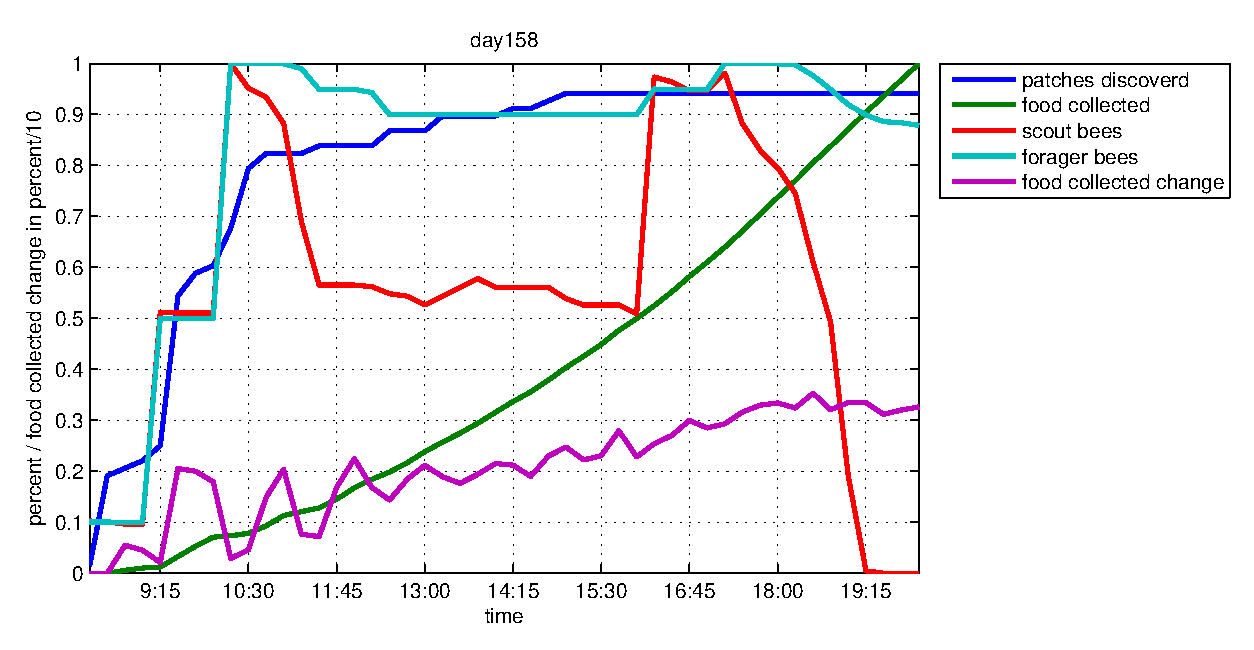
\includegraphics{../../code/results/Properties_Base_R1_1_day158.eps}}
			\caption{\textit{A summer day from the standard run R1\char`_1}}
			\label{fig:day158}
		\end{figure}
	 
	%TODO /PLANNED a summer day video / pictures	
	\subsubsection{Missing flower seasons}
	% summer and fall essential
	\subsubsection{Variations on autumn flowers}
	% we'll see what i find outd
	
	\subsubsection{Model restrictions}
	Even though we extended \textit{Khoury's} model by environmental influences on flowers and food reward, it is far from complete. One big divergence from nature is the treatment of pollen and nectar as one. Pollen, which is the protein source, and nectar, which is the carbohydrate source, are actually collected by two different forager classes intra-colonially \cite{schmickl07}.\\  Another big factor of disturbance are diseases and infections. Impairments in different aspects of a bee's life and behaviour, caused by pesticides or genetic mutation is entirely left out. There are also no other environmental influences such as aridity or wetland, human or invasive impacts of other species. \\
	Regarding the simulation of a bee's way of "thinking", we might never find a satisfying answer, it is only a model.   
	
